\documentclass{beamer}
\usepackage[utf8]{inputenc}
\usepackage{subcaption}
\usetheme{Madrid}

\institute[UAB]{Universitat Autònoma de Barcelona}
\title[Quants arbres generadors admet un graf?]{Arbre generador minimal. Quants arbres generadors admet un graf?}
\author[Víctor, Oriol, Eric, Carlo]{Víctor Ballester\and Oriol Bosquet \and Carlo Sala \and Eric Recio}
\date{Gener 2021}

\newtheorem{defin}[theorem]{Definició}

\begin{document}
\frame{\titlepage}
\AtBeginSection[]{
    \begin{frame}{Índex}
        \tableofcontents[currentsection]
    \end{frame}}
\section{Definicions prèvies}
\begin{frame}{Definicions prèvies}
    Comencem aquest treball definint els conceptes necessaris en relació amb els grafs i, en particular, amb els arbres.\pause
    \begin{defin}[Graf]
        \normalfont Un graf $G$ consisteix en una parella $(V(G), E(G))$ on:
        \begin{itemize}
            \item $V(G)$ és un conjunt (no buit) d'elements, anomenats vèrtexs del graf.
            \item $E(G)$ és un multiconjunt de parelles no ordenades de vèrtexs, que anomenem arestes del graf.
        \end{itemize}
    \end{defin}\pause
    \begin{defin}[Graf simple]
        \normalfont Sigui $G$ un graf. Diem que $G$ és simple si no té cap aresta múltiple (més d'una aresta entre els mateixos vèrtexs) ni bucles (arestes que van d'un vèrtex en ell mateix).
    \end{defin}
\end{frame}
\begin{frame}{Definicions prèvies}
    \begin{defin}[Multigraf]
        \normalfont Diem que $G$ és un multigraf si té, com a mínim, una aresta múltiple o bé un bucle.
    \end{defin}\pause
    Per conveni, quan parlem de grafs ens referirem a grafs simples. Quan vulguem considerar grafs que no siguin simples, ens hi referirem com a multigrafs.\pause
    \begin{defin}[Arbre]
        \normalfont Sigui $G$ un graf. Diem que $G$ és un arbre si $G$ és connex i no té cicles.
    \end{defin}\pause
    \begin{defin}[Fulla]
        \normalfont Sigui $T$ un arbre. Definim una fulla de $T$ com un vèrtex de grau 1.
    \end{defin}
\end{frame}
\begin{frame}{Definicions prèvies}
    \begin{defin}[Subgraf generador]
        \normalfont Sigui $G$ un graf connex. Un subgraf generador $G'$ de $G$ és un subgraf de $G$ tal que $V(G')=V(G)$. En particular, un arbre generador $T$ de $G$ és un subgraf generador de $G$ tal que $T$ és un arbre.
    \end{defin}\pause
    \begin{defin}[Matriu d'incidència]
        \normalfont Sigui $G$ un graf i sigui $n=|V(G)|$ i $m=|E(G)|$. La matriu d'incidència de $G$ és una matriu $M=(m_{ij})\in\mathcal{M}_{n\times m}(\mathbb{R})$ tal que:
        $$m_{ij}=\left\{\begin{array}{ll}
                1 & \text{si l'aresta $j$ és incident amb el vèrtex $i$,} \\
                0 & \text{altrament.}
            \end{array}\right.$$
    \end{defin}\pause
    Observem que la matriu d'incidència d'un graf tindrà exactament dos 1 en cada columna. Això ens condueix a definir la següent matriu.
\end{frame}
\begin{frame}{Definicions prèvies}
    \begin{defin}[Matriu d'incidència orientada]
        \normalfont Sigui $G$ un graf i $M$ la seva matriu d'incidència. Definim la matriu d'incidència orientada $M'$ de $G$ com la matriu $M$ on a cada columna canviem exactament un $1$ per un $-1$.
    \end{defin}\pause
    Per no fer un abús de notació, a partir d'ara denotarem per $M$ la matriu d'incidència orientada.\pause\space Fixem-nos que en aquesta matriu una de les files és supèrflua, ja que coneixent totes les altres i tenint en compte que en cada columna hi ha exactament un 1 i un $-1$, podem deduir què contindrà aquesta fila en qüestió. Això dona lloc a definir la següent matriu.\pause
    \begin{defin}[Matriu d'incidència orientada reduïda]
        \normalfont Sigui $G$ un graf i $M$ la seva matriu d'incidència orientada. Definim la matriu d'incidència orientada reduïda $M_0$ com la matriu $M$ en la qual s'ha eliminat una fila.  En aquest treball, per conveni, eliminarem sempre la darrera fila.
    \end{defin}
\end{frame}
\begin{frame}{Definicions prèvies}
    Per simplificar l'escriptura, d'ara endavant ens referirem a la matriu d'incidència orientada reduïda simplement com a matriu d'incidència reduïda, entenent que és la matriu amb 1's i $-1$'s.\pause
    \begin{defin}
        \normalfont Sigui $G$ un graf, $M_0$ la seva matriu d'incidència reduïda i $T$ un arbre generador de $G$. Definim la matriu d'incidència reduïda de $T$ com la matriu quadrada $M_0[T]$ obtinguda seleccionant les $n-1$ columnes de $M_0$ corresponents a les arestes de $T$ en $G$.
    \end{defin}
\end{frame}
\begin{frame}{Definicions prèvies}
    \begin{defin}[Matriu de Laplace]
        \normalfont Sigui $G$ un graf i sigui $n=|V(G)|$. Definim la matriu de Laplace $L=(\ell_{ij})\in\mathcal{M}_n(\mathbb{R})$ com:
        $$\ell_{ij}=\left\{\begin{array}{cl}
                \deg v_i & \text{si $i=j$,}                                   \\
                -1       & \text{si els vèrtexs $v_i$ i $v_j$ són adjacents,} \\
                0        & \text{altrament.}
            \end{array}\right.$$
    \end{defin}\pause
    Per clarificar aquestes definicions, posem un exemple on calculem totes les matrius que hem definit.
\end{frame}
\begin{frame}{Definicions prèvies}
    \begin{exampleblock}{Exemple}
        Sigui $G$ el graf de la figura.
        \begin{figure}
            \centering
            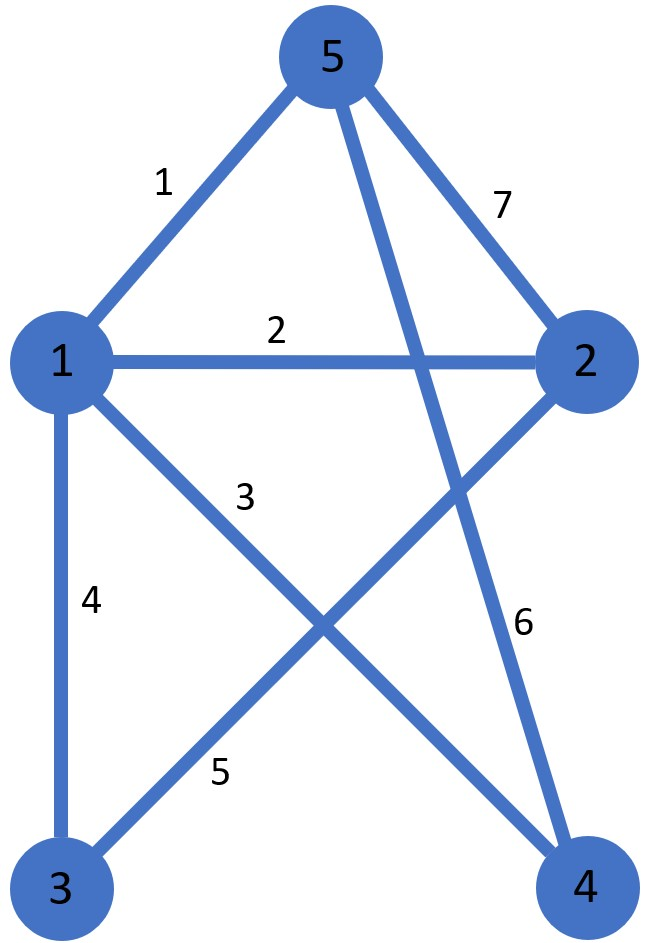
\includegraphics[width=4cm]{Imatges/exemple1.jpg}
        \end{figure}
    \end{exampleblock}
\end{frame}
\begin{frame}{Definicions prèvies}
    \begin{exampleblock}{}
        \begin{figure}
            \centering
            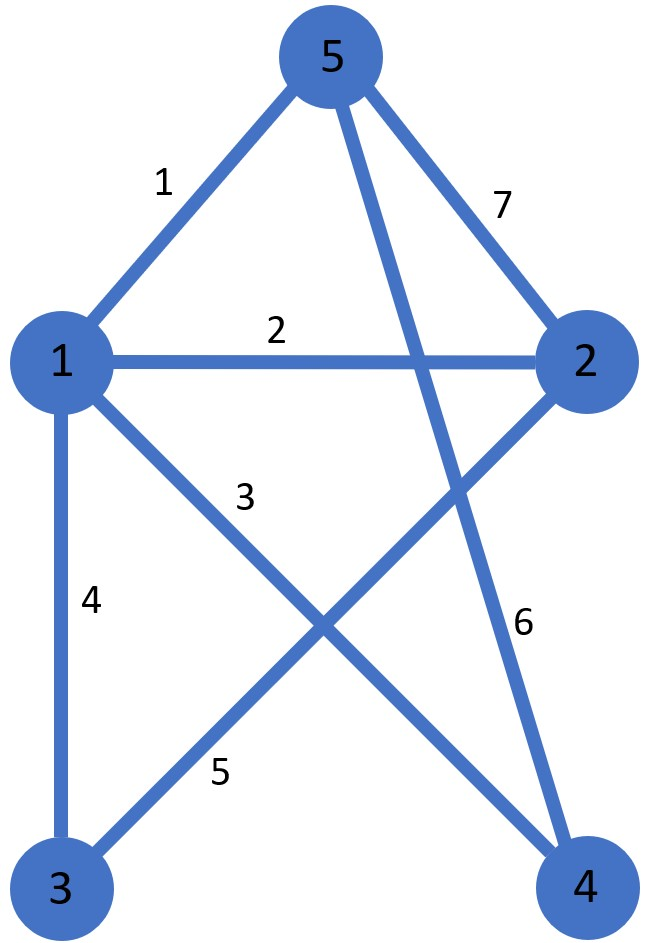
\includegraphics[width=2cm]{Imatges/exemple1.jpg}
        \end{figure}Aquest graf té les següents matrius associades:\pause\par
        \only<2>{Matriu d'incidència:
            $$\Tilde{M}=
                \begin{pmatrix}
                    1 & 1 & 1 & 1 & 0 & 0 & 0 \\
                    0 & 1 & 0 & 0 & 1 & 0 & 1 \\
                    0 & 0 & 0 & 1 & 1 & 0 & 0 \\
                    0 & 0 & 1 & 0 & 0 & 1 & 0 \\
                    1 & 0 & 0 & 0 & 0 & 1 & 1
                \end{pmatrix}.
            $$}
        \only<3>{Matriu d'incidència orientada:
            $$M=
                \begin{pmatrix}
                    1  & 1  & 1  & 1  & 0  & 0  & 0  \\
                    0  & -1 & 0  & 0  & 1  & 0  & 1  \\
                    0  & 0  & 0  & -1 & -1 & 0  & 0  \\
                    0  & 0  & -1 & 0  & 0  & 1  & 0  \\
                    -1 & 0  & 0  & 0  & 0  & -1 & -1
                \end{pmatrix}.
            $$}
        \only<4>{Matriu d'incidència orientada reduïda:
            $$M_0=
                \begin{pmatrix}
                    1 & 1  & 1  & 1  & 0  & 0 & 0 \\
                    0 & -1 & 0  & 0  & 1  & 0 & 1 \\
                    0 & 0  & 0  & -1 & -1 & 0 & 0 \\
                    0 & 0  & -1 & 0  & 0  & 1 & 0
                \end{pmatrix}.
            $$}
        \only<5>{Matriu de Laplace:
            $$L=
                \begin{pmatrix}
                    4  & -1 & -1 & -1 & -1 \\
                    -1 & 3  & -1 & 0  & -1 \\
                    -1 & -1 & 2  & 0  & 0  \\
                    -1 & 0  & 0  & 2  & -1 \\
                    -1 & -1 & 0  & -1 & 3
                \end{pmatrix}.
            $$}
    \end{exampleblock}
\end{frame}
\begin{frame}{Definicions prèvies}
    \begin{exampleblock}{}
        Si considerem l'arbre generador $T$ de la figura següent,
        \begin{figure}
            \centering
            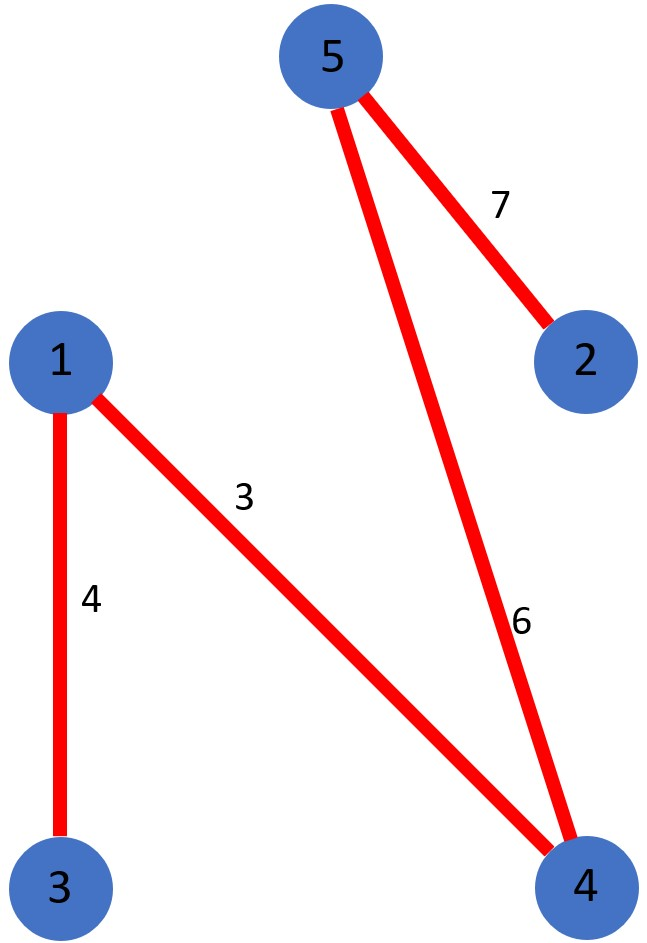
\includegraphics[width=2.45cm]{Imatges/exemple2.jpg}
        \end{figure}\pause
        la matriu d'incidència reduïda associada a l'arbre $T$ és:
        $$M_0[T]=
            \begin{pmatrix}
                1  & 1  & 0 & 0 \\
                0  & 0  & 0 & 1 \\
                0  & -1 & 0 & 0 \\
                -1 & 0  & 1 & 0
            \end{pmatrix}.
        $$
    \end{exampleblock}
\end{frame}

\section{Fórmula de Cayley}
\begin{frame}{Fórmula de Cayley}
    El 1889 Arthur Cayley va establir una fórmula per determinar el nombre d'arbres generadors diferents del graf complet $K_n$.\pause\space Hi ha moltes demostracions d'aquesta fórmula. En aquest treball en donarem una, presentada l'any 1918 pel matemàtic alemany Heinz Prüfer, establint una correspondència bijectiva entre arbres generadors amb $n$ vèrtexs i els anomenats codis de Prüfer (successions de longitud $n-2$). \pause\par Per tant, comencem definint la seqüència de Prüfer d'un arbre:
\end{frame}
\begin{frame}{Fórmula de Cayley}
    \begin{block}{Seqüència de Prüfer}
        Sigui $T$ un arbre d'ordre $n \geq 3$ amb conjunt de vèrtexs $V(T)= [n]$. Definim la seqüència de Prüfer com la successió
        $$\mathcal{P}(T)=(y_1,y_2,\ldots,y_{n-2})$$
        de $n-2$ nombres del conjunt $V(T)=[n]$.\pause\space Amb el següent algorisme, podem codificar qualsevol arbre en una seqüència de Prüfer:
        \begin{enumerate}
            \item Prenem la fulla de l'arbre $T$ amb etiqueta menor. Eliminem aquesta fulla de $T$ i li assignem el valor de l'etiqueta del seu únic vèrtex adjacent.
        \end{enumerate}
    \end{block}
\end{frame}
\begin{frame}{Fórmula de Cayley}
    \begin{block}{}
        \begin{enumerate}
            \setcounter{enumi}{1}
            \item Continuem el procés amb l'arbre creat a partir de $T$ en eliminar la fulla anterior i repetim l'algorisme fins que ens quedi un arbre d'un vèrtex.\pause\space Haurem obtingut una seqüència de $n-1$ nombres, que, descartant l'últim d'ells es transforma amb una seqüència de $n-2$ termes.
        \end{enumerate}
    \end{block}\pause
    Notem que aquesta seqüència d'un arbre és única.\pause\space En efecte, si $T$ és l'arbre considerat en qüestió i $\mathcal{P}(T)$ la seva seqüència de Prüfer, observem primer que les etiquetes de les fulles de $T$ no estan representades en $\mathcal{P}(T)$, ja que una fulla no pot ser adjacent a una altra fulla (considerant arbres d'ordre $n\geq 3$). Per tant, d'aquí es dedueix que cada vèrtex té grau igual a $1+a$, on $a$ és el nombre de vegades que apareix el vèrtex a $\mathcal{P}(T)$.\pause\par A la següent figura podem veure un exemple de com trobar la seqüència de Prüfer d'un arbre.
\end{frame}
\begin{frame}{Fórmula de Cayley}
    \begin{figure}[ht]
        \centering
        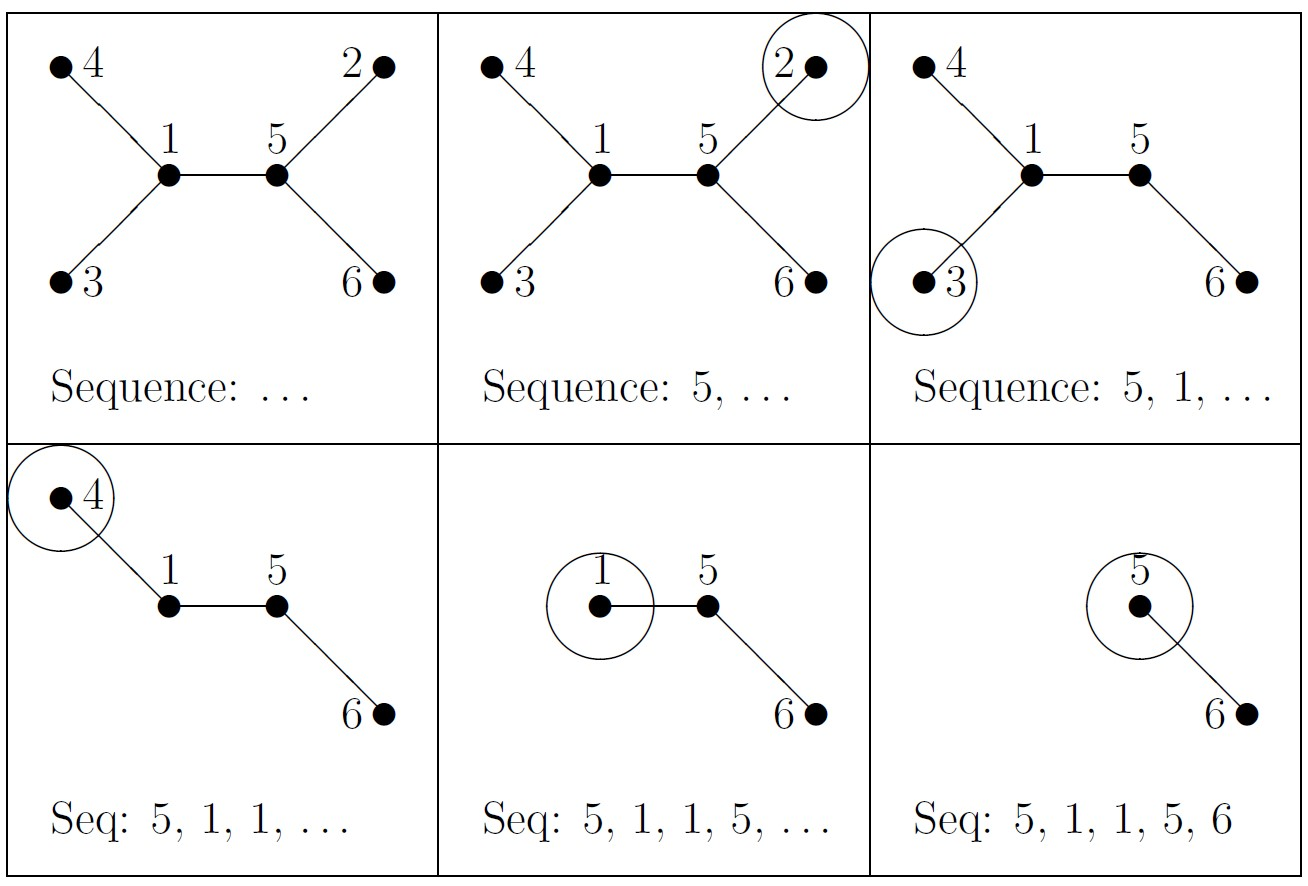
\includegraphics[width=9cm]{Imatges/prufer1.jpg}
    \end{figure}
\end{frame}
\begin{frame}{Fórmula de Cayley}
    El següent teorema ens diu que si tenim una seqüència de $n-2$ termes, automàticament també tenim un arbre $T$ amb seqüència de Prüfer igual a la que estàvem considerant.\pause
    \begin{alertblock}{Teorema}
        Sigui $T_n$ el conjunt d'arbres generadors d'ordre $n$ i $\mathcal{P}_n$ el conjunt de seqüències de Prüfer de $n-2$ termes. Considerem la següent aplicació de conjunts:
        \begin{align*}
            \varphi:T_n & \rightarrow \mathcal{P}_n \\
            T           & \mapsto \mathcal{P}(T)
        \end{align*}\pause
        Aleshores, $\varphi$ és bijectiva.
    \end{alertblock}
\end{frame}
\begin{frame}{Fórmula de Cayley}
    Ara sí, doncs, podem enunciar el teorema de Cayley:\pause
    \begin{alertblock}{Teorema de Cayley}
        Sigui $G=K_n$ un graf complet d'ordre $n\geq 2$. Aleshores hi ha $n^{n-2}$ arbres generadors diferents.
    \end{alertblock}\pause
    \begin{block}{Demostració}
        El cas $n=2$ és immediat.\pause\space Vegem el cas $n\geq3$.\par
        Pel teorema anterior sabem que el nombre de seqüència de Prüfer està en bijecció amb el nombre d'arbres generadors d'ordre $n$, per tant tindrem que $\tau(G):=|T_n|=|\mathcal{P}_n|$.\pause\space Ara bé, el conjunt $\mathcal{P}_n$ està format per paraules de longitud $n-2$ de l'alfabet $[n]$. Per tant, sabem que hi haurà $n^{n-2}$ paraules diferents i, per tant, tindrem que $\tau(G)=n^{n-2}$, tal com volíem demostrar.\qed
    \end{block}\pause
    Vegem ara un exemple d'aplicació de la fórmula de Cayley.
\end{frame}
\begin{frame}{Fórmula de Cayley}
    \begin{exampleblock}{Exemple}
        Considerem el graf complet $K_4$, és a dir, el graf de la següent figura.
        \begin{figure}[ht]
            \centering
            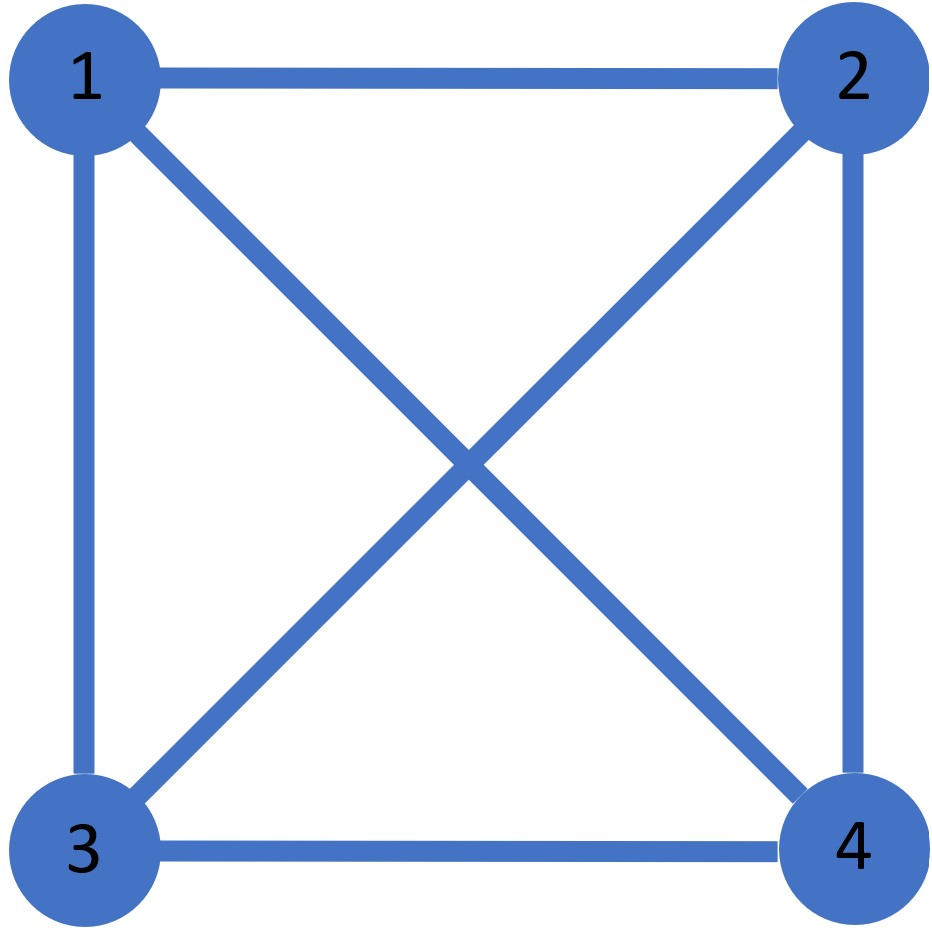
\includegraphics[width=4cm]{Imatges/graf2.jpg}
        \end{figure}\pause
        Per la fórmula de Cayley, el nombre d'arbres generadors és $4^{4-2} = 16$. A la figura següent els podem veure tots.
    \end{exampleblock}
\end{frame}
\begin{frame}{Fórmula de Cayley}
    \begin{exampleblock}{}
        \begin{figure}[ht]
            \centering
            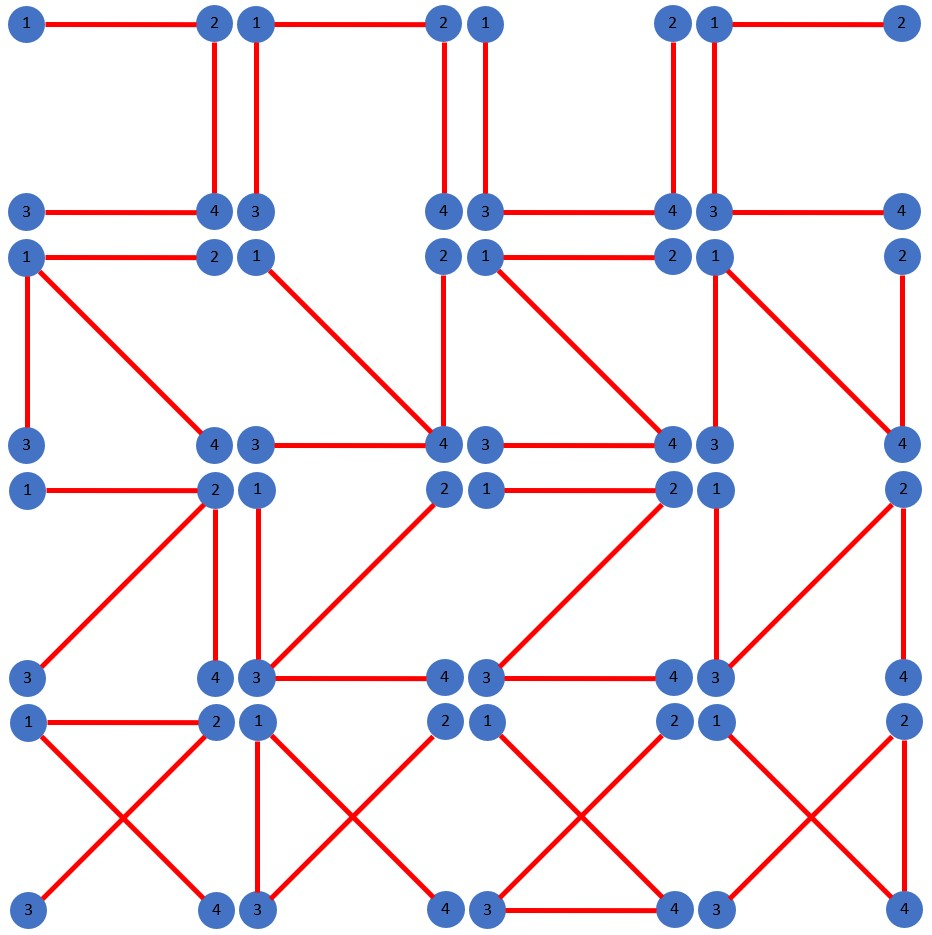
\includegraphics[width=7cm]{Imatges/graf2_16.jpg}
        \end{figure}
    \end{exampleblock}
\end{frame}

\section{Nombre d'arbres generadors}
\begin{frame}{Nombre d'arbres generadors}
    L'objectiu ara és generalitzar la fórmula de Cayley i calcular el nombre d'arbres generadors que tenim en un graf $G$ connex arbitrari. Per això, necessitem uns resultats previs.
    \pause
    \begin{block}{Lema}
        Sigui $G$ un graf connex d'ordre $n$. Si $M$ és la matriu d'incidència orientada de $G$ i $L$ és la matriu de Laplace de $G$, tenim que $$L=MM^t.$$
    \end{block}\pause
    \begin{alertblock}{Teorema}
        Sigui $G$ un graf i $T$ un subgraf de $G$. Aleshores, $T$ és un arbre generador de $G$ si i només si $|\det M_0[T]|=1$.
    \end{alertblock}
\end{frame}
\begin{frame}{Nombre d'arbres generadors}
    \begin{alertblock}{Fórmula de Cauchy-Binet}
        Sigui $A\in\mathcal{M}_{n\times m}(\mathbb{R})$ i $B\in\mathcal{M}_{m\times n}(\mathbb{R})$. Donat qualsevol subconjunt $S\subset\{1,\ldots,m\}$ tal que $|S|=n$, formem la matriu $A_S\in\mathcal{M}_n(\mathbb{R})$ escollint les columnes de $A$ indexades pel conjunt $S$ i formem la matriu $B_S\in\mathcal{M}_n(\mathbb{R})$ escollint les files de $B$ indexades pel conjunt $S$. Aleshores tenim que $$\det(AB)=\sum_S\det(A_S)\det(B_S).$$
    \end{alertblock}
\end{frame}
\begin{frame}{Nombre d'arbres generadors}
    Passem ara a enunciar el nombre d'arbres generadors d'un graf.\pause
    \begin{alertblock}{Teorema de Kirchhoff}
        Sigui $G$ un graf connex amb matriu de Laplace $L$. Sigui $n=|V(G)|$, $m=|E(G)|$ i sigui $L_i$ la matriu resultant d'haver tret a $L$ la fila i columna $i$-èssimes, per a qualsevol $i\in\{1,\ldots,n\}$.\pause\space Aleshores, el valor $\det L_i$ és independent de $i$ i el nombre $\tau(G)$ d'arbres generadors de $G$ és $$\tau(G)=\det L_i.$$
    \end{alertblock}\pause
    \begin{block}{Demostració}
        Com que $M_0$ l'hem creada suprimint l'última fila de $M$ ho demostrarem únicament per $L_0:=L_n$.\pause\par En un lema anterior hem vist que teníem la igualtat: $L=MM^t$. Aleshores, és clar que tindrem $L_0=M_0M_0^t$.
    \end{block}
\end{frame}
\begin{frame}{Nombre d'arbres generadors}
    \begin{block}{}
        Per la fórmula de Cauchy-Binet aplicat a les matrius $M_0$ i $M_0^t$ tenim que \begin{equation}
            \det L_0=\det(M_0M_0^t)=\sum_S\det((M_0)_S)\det((M_0^t)_S),
            \label{eq1}
        \end{equation} on $S\subset\{1,\ldots,m\}$ tal que $|S|=n$.\pause\space Ara bé, en general tenim que per una matriu $A\in\mathcal{M}_{p\times q}(\mathbb{R})$ es compleix $(A^t)_S=(A_S)^t$, i aleshores l'equació \ref{eq1} esdevé
        \begin{equation}
            \det L_0=\sum_S(\det(M_0)_S)^2.
            \label{eq2}
        \end{equation}\pause
        Ara bé, per un teorema anterior tenim que $(\det(M_0)_S)^2=1$ si les arestes indexades per $S$ defineixen un arbre generador de $G$ y $(\det((M_0)_S))^2=0$, en cas contrari.\pause\space Per tant, és clar que que la suma de l'equació \ref{eq2} compta el nombre total d'arbres generadors, és a dir, $\tau(G)=\det L_0$.\qed
    \end{block}
\end{frame}
\begin{frame}{Nombre d'arbres generadors}
    L'objectiu ara és trobar algun mètode alternatiu per al càlcul de $\tau(G)$.\pause
    \begin{alertblock}{Corol·lari}
        Sigui $G$ un graf connex tal que $n=|V(G)|$. Suposem que els valors propis de $L$ són $\lambda_1,\ldots,\lambda_n$, amb $\lambda_n=0$. Aleshores, $$\tau(G)=\frac{1}{n}\lambda_1\lambda_2\ldots\lambda_{n-1}.$$
    \end{alertblock}\pause
    Considerem ara el següent exemple:
\end{frame}
\begin{frame}{Nombre d'arbres generadors}
    \begin{exampleblock}{Exemple}
        Considerem el graf $G$ de la figura.
        \begin{figure}[ht]
            \centering
            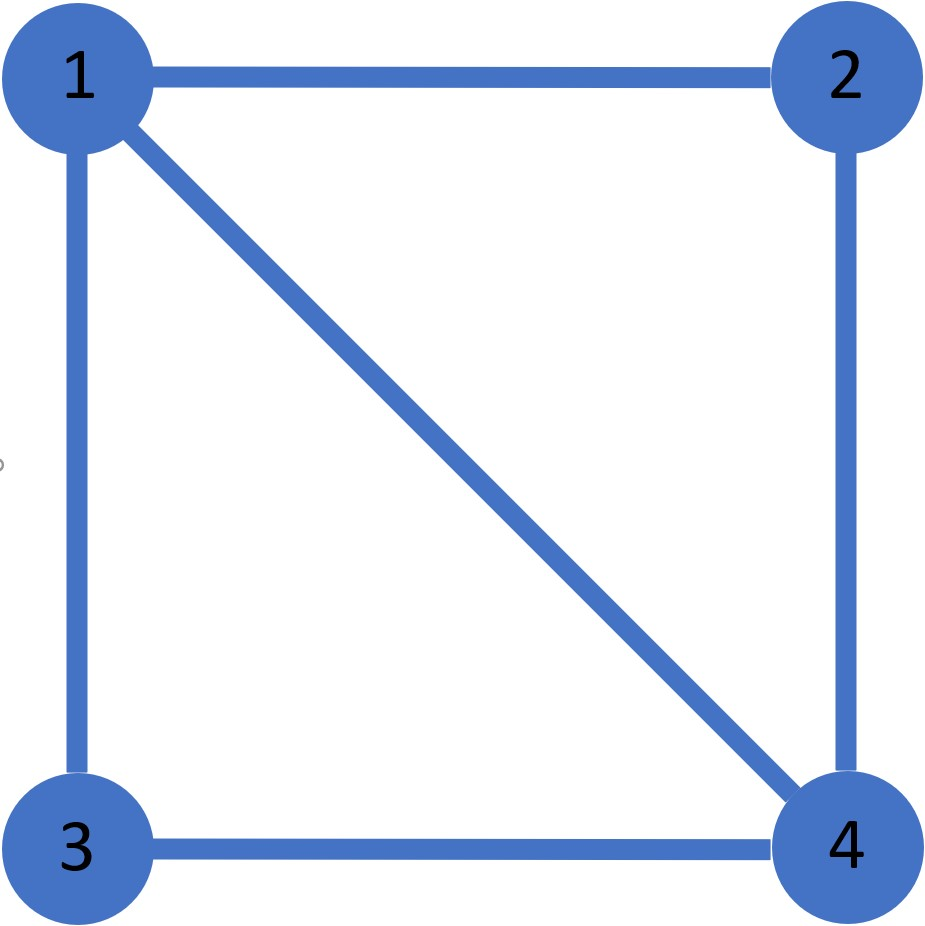
\includegraphics[width=4cm]{Imatges/graf1.jpg}
        \end{figure}
        Volem calcular el nombre d'arbres generadors d'aquest graf.\pause\space  Per això necessitem trobar la matriu de Laplace associada.
    \end{exampleblock}
\end{frame}
\begin{frame}{Nombre d'arbres generadors}
    \begin{exampleblock}{}
        \begin{figure}
            \centering
            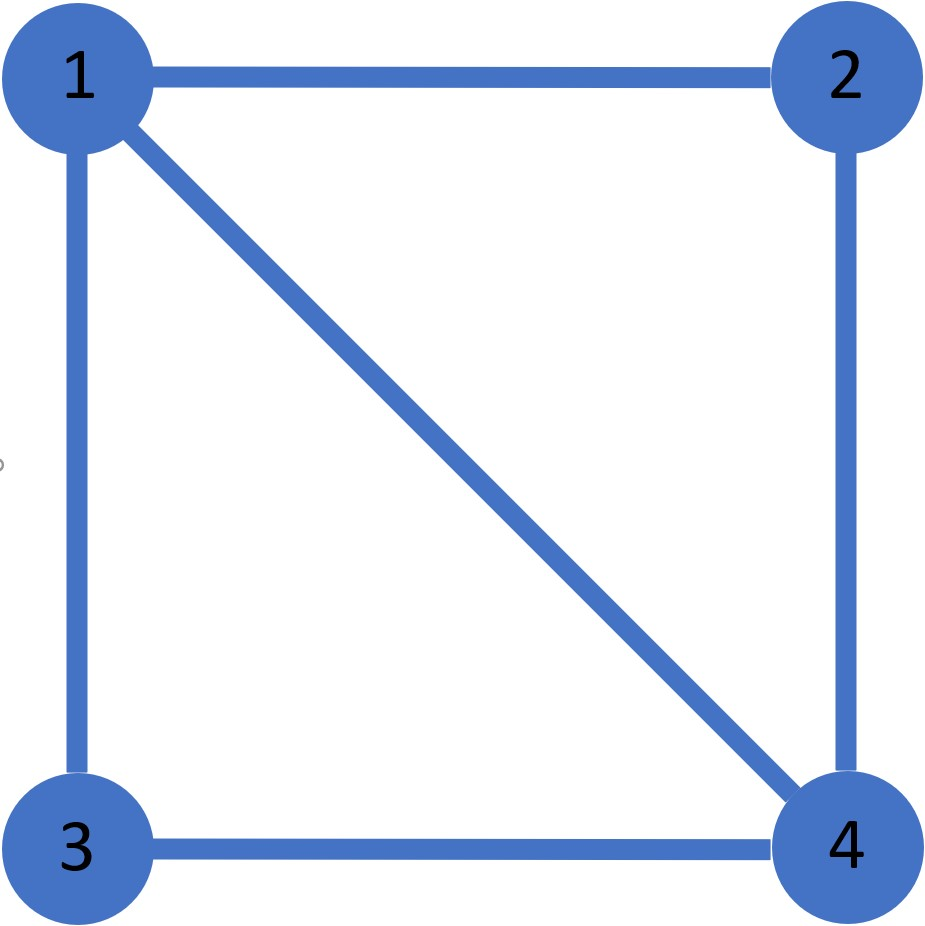
\includegraphics[width=2.5cm]{Imatges/graf1.jpg}
        \end{figure}
        En aquest cas tenim que $$L=\begin{pmatrix}
                3  & -1 & -1 & -1 \\
                -1 & 2  & 0  & -1 \\
                -1 & 0  & 2  & -1 \\
                -1 & -1 & -1 & 3  \\
            \end{pmatrix}.$$\pause
        Calcularem el valor de $\tau(G)$ mitjançant els dos mètodes que hem exposat.
    \end{exampleblock}
\end{frame}
\begin{frame}{Nombre d'arbres generadors}
    \begin{exampleblock}{}
        \begin{enumerate}
            \item Utilitzant el teorema de Kirchhoff, podem crear $L_0$ suprimint la primera fila i columna de $L$.\pause\space Així tenim que $$\tau(G)=\det L_0=\begin{vmatrix}
                          2  & 0  & -1 \\
                          0  & 2  & -1 \\
                          -1 & -1 & 3  \\
                      \end{vmatrix}=8.$$\pause
            \item Utilitzant el mètode dels valors propis hem de calcular el polinomi característic de $L$.\pause\space Tenim doncs que:
                  $$\det(L-xI)=\begin{vmatrix}
                          3-x & -1  & -1  & -1  \\
                          -1  & 2-x & 0   & -1  \\
                          -1  & 0   & 2-x & -1  \\
                          -1  & -1  & -1  & 3-x \\
                      \end{vmatrix}=$$
        \end{enumerate}
    \end{exampleblock}
\end{frame}
\begin{frame}{Nombre d'arbres generadors}
    \begin{exampleblock}{}
        \begin{multline*}
            =\begin{vmatrix}
                -x & -1  & -1  & -1  \\
                -x & 2-x & 0   & -1  \\
                -x & 0   & 2-x & -1  \\
                -x & -1  & -1  & 3-x \\
            \end{vmatrix}=-x\begin{vmatrix}
                1 & -1  & -1  & -1  \\
                1 & 2-x & 0   & -1  \\
                1 & 0   & 2-x & -1  \\
                1 & -1  & -1  & 3-x \\
            \end{vmatrix}=\\=-x\begin{vmatrix}
                1 & 0   & 0   & 0   \\
                1 & 3-x & 1   & 0   \\
                1 & 1   & 3-x & 0   \\
                1 & 0   & 0   & 4-x \\
            \end{vmatrix}=-x(4-x)[(3-x)^2-1]=\\=x(x-2)(x-4)^2.
        \end{multline*}\pause
        Per tant, els valors propis de $L$ són $\lambda_1=2$, $\lambda_2=\lambda_3=4$ i $\lambda_4=0$.\pause\space  Finalment, tenim que $$\tau(G)=\frac{1}{4}\lambda_1\lambda_2\lambda_3=8.$$
    \end{exampleblock}
\end{frame}
\begin{frame}{Nombre d'arbres generadors}
    \begin{exampleblock}{}
        En la següent figura observem els 8 arbres generadors del graf $G$.
        \begin{figure}[ht]
            \centering
            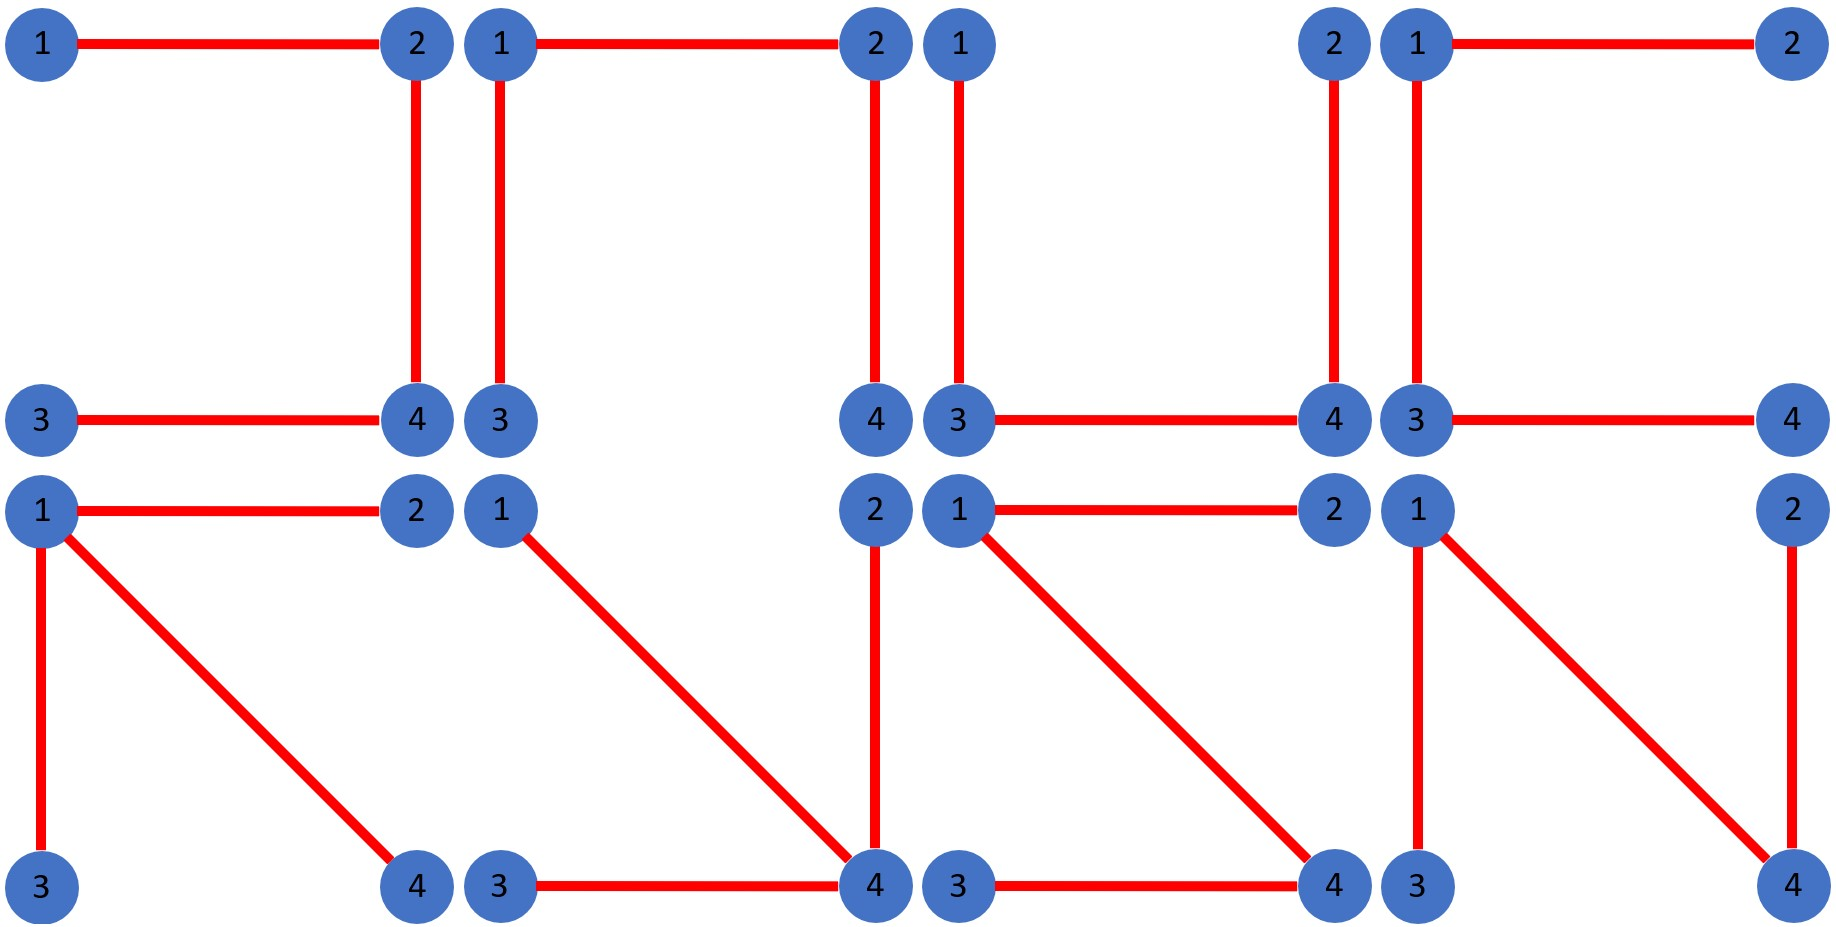
\includegraphics[width=9cm]{Imatges/graf1_8.jpg}
        \end{figure}\pause
        Observem que el graf considerat en aquest exemple és un subgraf del graf $K_4$ i, evidentment, tots els seus arbres generadors són arbres generadors del graf $K_4$.
    \end{exampleblock}
\end{frame}

\section{Aplicacions}
\begin{frame}{Aplicacions}
    Ara aplicarem aquests conceptes a una aplicació en particular: trobar l'arbre generador minimal d'un graf. Per això necessitem definir uns quants conceptes.\pause
    \begin{block}{Definició}
        Donat un graf $G$, diem que aquest és un graf ponderat, pesat o amb costos quan les arestes tenen associades un valor, és a dir, per a tot $e\in E(G)$ considerem el cost $w(e)$ associat a l'aresta $e$.
    \end{block}\pause
    \begin{block}{Definició}
        Donat un graf $G$ ponderat per una funció $w(e)$ i un arbre generador $T$ de $G$ definim el pes de l’arbre $T$ com $$w(T)=\sum_{e\in E(G)} w(e).$$
    \end{block}
\end{frame}
\begin{frame}{Aplicacions}
    \begin{block}{Definició}
        Un arbre generador minimal, o de cost mínim, de $G$ és un arbre generador $T$ de $G$ de pes $w(T)$ mínim.
    \end{block}\pause
    Per tal de determinar l’arbre generador de cost mínim d’un graf, farem ús de diferents algoritmes en funció de les característiques del graf. A continuació, exposem de manera detallada dos algoritmes per grafs connexos, no dirigits i ponderats d’ordre $n$ i mida $m$.
\end{frame}
\begin{frame}{Aplicacions}
    \begin{alertblock}{Algoritme de Prim}
        Sigui $G$ un graf. Per crear l'arbre generador de cost mínim seguim els següents passos:
        \begin{enumerate}
            \item Escollim un vèrtex $v_1\in V(G)$ i considerem l’arbre $T$ format pel vèrtex $v_1$.\pause
            \item Sigui $e'$ l’aresta de pes mínim incident a un vèrtex de $T$ i un altre vèrtex $u\notin V(T)$. A continuació, creem el nou arbre $T:=T+e'$.\pause
            \item Si $|E(T)|=n-1$ ja hem acabat. Si no, tornem al pas 2.
        \end{enumerate}\pause
    \end{alertblock}
    Observem que l’elecció del vèrtex inicial pot fer que l’arbre generat sigui diferent, però en qualsevol cas serà de cost mínim.\pause \par L’algoritme de Prim té una complexitat de $O(n^2)$.
\end{frame}
\begin{frame}{Aplicacions}
    \begin{alertblock}{Algoritme de Kruskal}
        Sigui $G$ un graf. La descripció de l'obtenció de l'arbre generador de cost mínim a través de l'algoritme de Kruskal és la següent:
        \begin{enumerate}
            \item Escollim l'aresta de pes mínim $e$ i considerem l'arbre $T$ format per aquesta aresta.\pause
            \item Sigui $e'$ l’aresta de pes mínim tal que $e'\notin E(T)$ i $T+e'$ no forma cap cicle. Aleshores, considerem el nou graf $T:=T+e$.\pause
            \item Si $|E(T)|=n-1$ ja hem acabat. Si no, tornem al pas 2.
        \end{enumerate}
    \end{alertblock}\pause
    L’algoritme de Kruskal té una complexitat de $O(m\log m)$.
\end{frame}
\begin{frame}{Aplicacions}
    Arribats en aquest punt, ens preguntem quin dels algoritmes és més eficient o quin convé utilitzar. \pause La resposta és que depèn del nombre d’arestes del graf.\pause
    \begin{itemize}
        \item<3-> Si $|E(G)|\sim |E(K_n)|$, aleshores $$|E(G)|= O(n^2)\implies\left\{\begin{array}{cc}
                      \text{Prim:}    & O(n^2)       \\
                      \text{Kruskal:} & O(n^2\log n)
                  \end{array}\right\}.$$\pause Per tant, convé utilitzar l'algoritme de Prim.\pause
        \item<4-> Si $|E(G)|\sim |V(K_n)|$, aleshores $$|E(G)|= O(n)\implies\left\{\begin{array}{cc}
                      \text{Prim:}    & O(n^2)     \\
                      \text{Kruskal:} & O(n\log n)
                  \end{array}\right\}.$$\pause Per tant, convé utilitzar l'algoritme de Kurskal.
    \end{itemize}
\end{frame}
\end{document}

